\section*{Conclusiones}
\vspace{2ex}
Los resultados del an\'alisis y s\'intesis del filtro \textit{Pasa Altos} se corroboran entre el m\'etodo anal\'itico, la simulaci\'on y luego con las mediciones realizadas. Si bien hubo que tomar comporomisos a la hora de armar el circuito y elegir valores de componenetes estandarizados, por optimizaron las diferencias entre la frecuencia de corte $f_0$ y el factor de selectividad $Q$, optandose por dejar que este aumente en pos de mantener la diferencia conjunta lo mas baja posible. Esto permitio tener una frecuencia de corte virtualmente identica a la ideal y obtener en las mediciones resultados muy favorables, indicando que el filtro diseñado cumple aceptablemente con las especificaciones propuestas en la consigna del trabajo pr\'actico. Adjunto unas ultimas imagenes para comparar el total de los resultados de la. respuesta en frecuencia
\begin{centering}
	\begin{figure}[h]
		\centering
		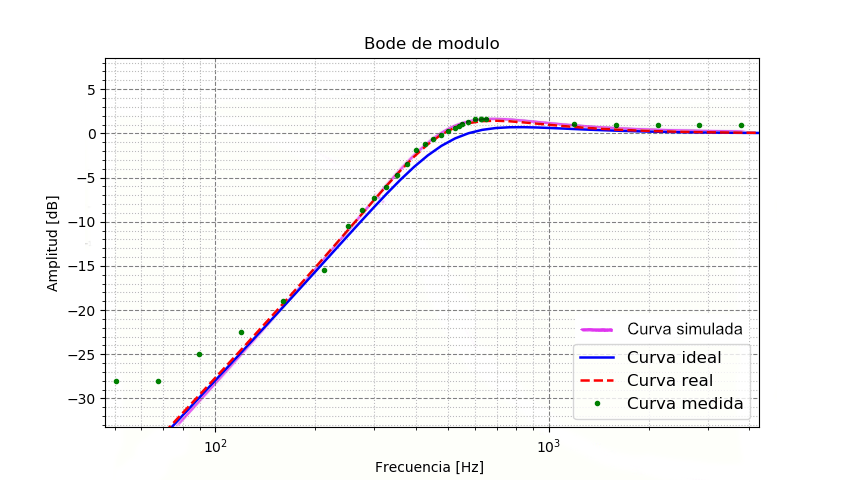
\includegraphics[width=1\textwidth]{imagenes/ComparativaFinal.png}
		\caption{Total de los resultados de respuesta en frecuencia del filtro}
		
	\end{figure}	
\end{centering}
